\documentclass[14pt]{article}
\usepackage[utf8]{inputenc}  % To handle UTF-8 encoding
\usepackage[vietnamese]{babel}  % To handle Vietnamese text
\usepackage{graphicx}
\usepackage{setspace}
\usepackage{fancyhdr}
\pagestyle{fancy}
\fancyhf{}
\fancyfoot[R]{\thepage}
\usepackage{pifont}
\usepackage{tikz}
\usepackage{mathptmx}
\usepackage{titlesec}
\usepackage[backend=biber,style=ieee]{biblatex}
\addbibresource{references.bib}  % Thêm tệp .bib chứa các nguồn tham khảo của bạn
\usepackage{tocloft}   % For \addcontentsline
\usepackage[left=3cm,right=2cm,top=2cm,bottom=2cm]{geometry}
\usepackage{setspace}
\usepackage[T1]{fontenc}
\usepackage{array}
\usepackage{booktabs}
\setstretch{1.5}
% 
\renewcommand{\baselinestretch}{1.5}


\graphicspath{{./images/}}
% Điều chỉnh kích thước font cho \subsection
\titleformat{\subsection}
  {\normalfont\fontsize{14}{15}\selectfont\bfseries} % 12pt font size, 15pt line spacing, in bold
  {\thesubsection}{1em}{}

% Điều chỉnh kích thước font cho \subsubsection
\titleformat{\subsubsection}
  {\normalfont\fontsize{14}{13}\selectfont\bfseries} % 10pt font size, 13pt line spacing, in bold
  {\thesubsubsection}{1em}{}

\makeatletter
\renewcommand{\tableofcontents}{%
    \@starttoc{toc}%
}
\renewcommand{\listoffigures}{%
    \@starttoc{lof}%
}

\makeatother

\begin{document}
\onehalfspacing
%------------------------------------------------------------
%|						COVER PAGE						
%------------------------------------------------------------
% Vẽ khung cho trang đầu tiên

\begin{center}
	\pagenumbering{gobble}
	\fontsize{16}{20}\selectfont
	\textbf{TRƯỜNG ĐẠI HỌC CÔNG THƯƠNG TP.HỒ CHÍ MINH\\ 
		\textbf{KHOA CÔNG NGHỆ THÔNG TIN}}
	
	\vspace{0.8cm}
	\begin{figure}[htp]
		\begin{center}
			\includegraphics[scale=0.08]{images/logo.png}
		\end{center}
	\end{figure}
	\vspace{1cm}
	\fontsize{24}{20}\selectfont\textbf{BÁO CÁO THỰC TẬP TỐT NGHIỆP\\}
	
	\vspace{3cm}
	\fontsize{24}{20}\selectfont\textbf{ỨNG DỤNG YOLO VÀ OPENCV THIẾT KẾ HỆ THỐNG PHÁT HIỆN CON NGƯỜI VÀ ĐÁNH GIÁ AN TOÀN}
\end{center}
\vspace{2cm}
\begin{center}
	\fontsize{14}{20}\selectfont\textit{}{Sinh viên thực hiện: HOÀNG THẾ ANH}\\
	\fontsize{14}{20}\selectfont\textit{}{Mã sinh viên: 2001202008 Lớp: 11DHTH9}

\end{center}
\pagebreak    
%------------------------------------------------------------
%|						COVER PAGE						
%------------------------------------------------------------
% Vẽ khung cho trang đầu tiên

\begin{center}
	\pagenumbering{gobble}
	\fontsize{16}{20}\selectfont
	\textbf{TRƯỜNG ĐẠI HỌC CÔNG THƯƠNG TP.HỒ CHÍ MINH\\ 
		\textbf{KHOA CÔNG NGHỆ THÔNG TIN}}
	
	\vspace{0.8cm}
	\begin{figure}[htp]
		\begin{center}
			\includegraphics[scale=0.08]{images/logo.png}
		\end{center}
	\end{figure}
	\vspace{1cm}
	\fontsize{24}{20}\selectfont\textbf{BÁO CÁO THỰC TẬP TỐT NGHIỆP\\}
	
	\vspace{3cm}
	\fontsize{24}{20}\selectfont\textbf{ỨNG DỤNG YOLO VÀ OPENCV THIẾT KẾ HỆ THỐNG PHÁT HIỆN CON NGƯỜI VÀ ĐÁNH GIÁ AN TOÀN}
\end{center}
\vspace{2cm}
\begin{center}
	\fontsize{14}{20}\selectfont\textit{}{Sinh viên thực hiện: HOÀNG THẾ ANH}\\
	\fontsize{14}{20}\selectfont\textit{}{Mã sinh viên: 2001202008 Lớp: 11DHTH9}

\end{center}
\pagebreak
	%------------------------------------------------------------
	%|					CAM ĐOAN PAGE					|
	%------------------------------------------------------------
    \pagestyle{fancy}
	\fancyhf{}
	\chead{\thepage}
	\renewcommand{\headrulewidth}{0pt}
	\begin{center}
		\pagenumbering{roman}\setcounter{page}{1}
		\fontsize{16}{20}\selectfont
		\textbf{LỜI CAM ĐOAN\\} 
	\end{center}
	\setstretch{1.5}
	\fontsize{13}{13}\selectfont
	\paragraph{}
	Tôi xin cam đoan đây là công trình nghiên cứu của riêng tôi. Các số liệu, kết quả nêu trong Báo cáo thực tập tốt nghiệp là trung thực và chưa từng được ai công bố trong bất kỳ công trình nào khác.
	\paragraph{}
    	Tôi xin cam đoan rằng mọi sự giúp đỡ cho việc thực hiện Báo cáo thực tập tốt nghiệp này 
    đã được cảm ơn và các thông tin trích dẫn trong Báo cáo thực tập tốt nghiệp đã được chỉ rõ nguồn gốc.
	
	\begin{flushright}
            \textbf {Sinh viên thực hiện báo cáo} \\
            \textit{(Ký và ghi rõ họ tên)}
        \end{flushright}
	\pagebreak	
	%------------------------------------------------------------
	%|					ACKNOWLEDGEMENT PAGE					|
	%------------------------------------------------------------
	\pagestyle{fancy}
	\fancyhf{}
	\chead{\thepage}
	\renewcommand{\headrulewidth}{0pt}
	\begin{center}
		\pagenumbering{roman}\setcounter{page}{1}
		\fontsize{16}{20}\selectfont
		\textbf{LỜI CẢM ƠN\\} 
	\end{center}
	\setstretch{1.5}
	\fontsize{13}{13}\selectfont
	\paragraph{}
	Trong thời gian thực tập tại công ty TNHH LUNA NEXUS VN INC., em xin cảm ơn quý công ty đã tạo điều kiện để em có thể hoàn thành được kì thực tập của mình.
	\paragraph{}
	Xin cảm ơn Kĩ sư Trần Minh Vương, anh là người trực tiếp giám sát quá trình thực tập cũng như là người hỗ trợ em tìm kiếm tài liệu chuyên ngành và giải đáp các thắc mắc về dự án thực tập trong suốt quá trình làm việc tại công ty.

	\paragraph{}
	Em xin chân thành cảm ơn Trường Đại học Công Thương Thành phố Hồ Chí Minh đã tạo điều kiện để em có thể được trực tiếp học tập ở doanh nghiệp và thu được nhiều bài học cũng như là kinh nghiệm quý báu trong quá trình làm việc.
	\paragraph{}
	Cảm ơn gia đình, những người bạn học đã luôn cổ vũ mình và tạo điều kiện giúp cho mình có thể hoàn thành tốt được dự án thực tập tại học kì doanh nghiệp.
	\paragraph{}
	Em xin cảm ơn.
	\pagebreak	

	%------------------------------------------------------------
	%|					TABLEOFCONTENT PAGE						|
	%------------------------------------------------------------
	\begin{center}
		\pagenumbering{arabic}\setcounter{page}{1}
		\fontsize{16}{20}\selectfont
		\textbf{MỤC LỤC\\} 
		
	\end{center}
	\setstretch{1.5}
	\fontsize{13}{13}\selectfont
	\tableofcontents
	\addcontentsline{toc}{section}{LỜI CẢM ƠN}
	
	
	
	
	
	\pagebreak

	%------------------------------------------------------------
	%|					List Of Figure PAGE						|
	%------------------------------------------------------------
	\begin{center}
		\pagenumbering{arabic}\setcounter{page}{1}
		\fontsize{16}{20}\selectfont
		\textbf{DANH MỤC HÌNH ẢNH\\} 
		
	\end{center}
	\setstretch{1.5}
	\fontsize{13}{13}\selectfont
	\listoffigures
	
	
	\pagebreak
	%------------------------------------------------------------
	%|					CHAPTER 1		                     	|  
	%| GIỚI THIỆU CHUNG ĐƠN VỊ THỰC TẬP              			|
	%------------------------------------------------------------
	\begin{center}
		\pagenumbering{arabic}\setcounter{page}{2}
	\end{center}
	
	\begin{flushleft}
		
		\fontsize{16}{20}\selectfont
		\section*{CHƯƠNG 1: GIỚI THIỆU CHUNG ĐƠN VỊ THỰC TẬP }
		\addcontentsline{toc}{section}{CHƯƠNG 1: GIỚI THIỆU CHUNG ĐƠN VỊ THỰC TẬP }
		\fontsize{13}{13}\selectfont
		%
		% Phần 1
		%
        \setcounter{section}{1}


        \subsection{Thông tin về đơn vị thực tập}
		\subsubsection{Sơ lược về sự hình thành và phát triển của đơn vị}
		\subsubsection{Tổ chức và các lĩnh vực hoạt động của đơn vị}
		\subsubsection{Tổ chức quản lý sử dụng các nguồn lực của đơn vị}
		\subsubsection{Cơ cấu tổ chức}
		\subsubsection{Tình hình hoạt động kinh doanh của doanh nghiệp}

		\subsection{Thông tin về vị trí sinh viên tham gia thực tập}
		\subsubsection{Giới thiệu chung về vị trí công tác}
		\subsubsection{Đặc điểm, yêu cầu}
		\subsubsection{Cơ cấu tổ chức, nhiệm vụ liên quan}
	%------------------------------------------------------------
	%|					CHAPTER 2		                     	|  
	%| PHÂN TÍCH THỰC TRẠNG CỦA VẤN ĐỀ CÓ LIÊN QUAN ĐẾN
    %| ĐỀ TÀI MÀ SINH VIÊN CHỌN VIẾT BÁO CÁO THỰC TẬP TẠI DOANH NGHIỆP THỰC TẬP             			|
	%------------------------------------------------------------
	\pagestyle{fancy}
	\fancyhf{}
	\fancyfoot[R]{\thepage}
\begin{flushleft}
    \fontsize{16}{20}\selectfont
    \section*{CHƯƠNG 2: PHÂN TÍCH THỰC TRẠNG CỦA VẤN ĐỀ CÓ LIÊN QUAN ĐẾN
    ĐỀ TÀI MÀ SINH VIÊN CHỌN VIẾT BÁO CÁO THỰC TẬP TẠI DOANH NGHIỆP THỰC TẬP}
    \addcontentsline{toc}{section}{CHƯƠNG 2: PHÂN TÍCH THỰC TRẠNG CỦA VẤN ĐỀ CÓ LIÊN QUAN ĐẾN
    ĐỀ TÀI MÀ SINH VIÊN CHỌN VIẾT BÁO CÁO THỰC TẬP TẠI DOANH NGHIỆP THỰC TẬP}
    \fontsize{13}{20}\selectfont
    \paragraph{}
    \fontsize{13}{20}\selectfont Trong quá trình thực tập tại công ty, em đã được giao dự án về phát triển phần mềm sử dụng YOLO và OpenCV để xác định và đưa ra cảnh báo đối với các đối tượng là con người trong một khu vực cụ thể.\\
    \setcounter{section}{2}
    \setcounter{subsection}{0}
    
    \subsection{Giải Pháp}
    \fontsize{13}{13}\selectfont\paragraph{}
    Để giải quyết các vấn đề trên, mô hình nhận diện đối tượng YOLO và bộ OpenCV được úng dụng vào giải pháp theo dõi con người và đánh giá an toàn. \\
    
    \subsection{Phân tích đánh giá tình hình thực tế theo chủ đề thực tập tại đơn vị}
    \subsubsection{Vấn Đề Đặt Ra}
    \fontsize{13}{20}\selectfont Vấn đề được đặt ra là phải làm sao để có thể xác định được chủ thể con người trong camera (Camera an ninh, điện thoại,...) và xác nhận xem chủ thể có ở trong khu vực được đánh dấu là an toàn hay không, vấn đề này có thể được áp dụng vào các tình huống trong đời sống hàng ngày cũng như trong doanh nghiệp, sản xuất:\\ 
    \begin{itemize}
        \item Trong gia đình: \\
        Bài toán này có thể giúp phụ huynh có thể trông con em mình, ví dụ như thông qua camera giám sát và các điểm thiết lập đã được cài đặt sẵn,phụ huynh có thể giám sát được xem là trẻ có đang trong khu vực an toàn hay không,...
        \begin{figure}[htbp]
            \centering
            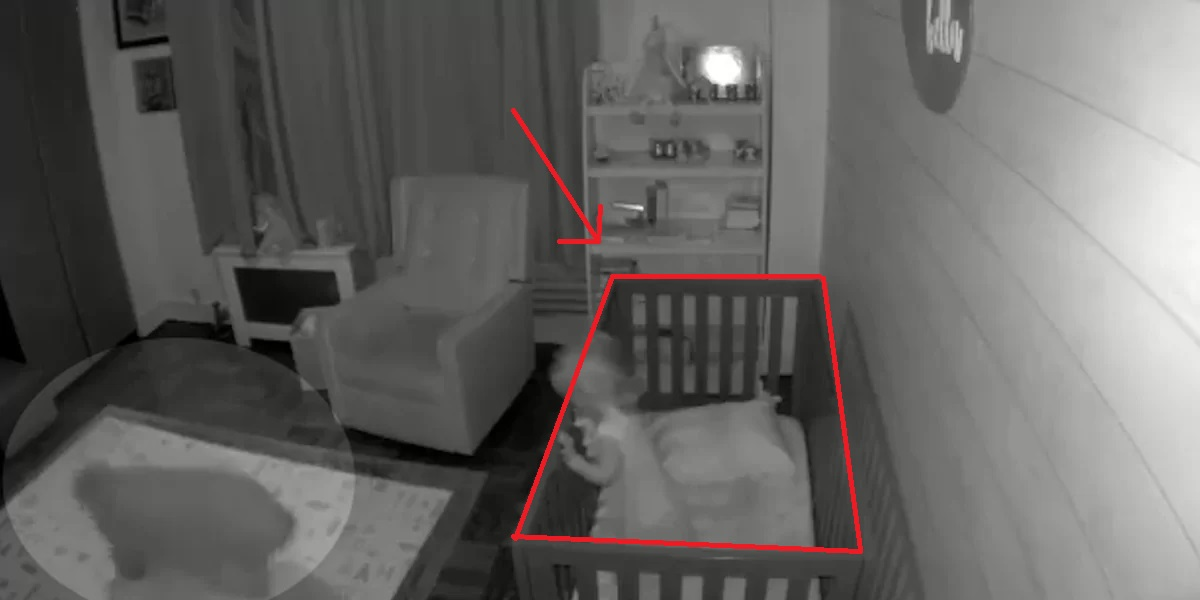
\includegraphics[width=0.5\textwidth]{images/TH1.jpg}
            \caption{Trong trường hợp gia đình.}
            \label{fig:img_1_GD}
        \end{figure}
        \item Trong văn phòng:\\
        Trong văn phòng, có thể giám sát xem, nhân viên có đang làm việc trong khu vực chỉ định hay không,...
        \begin{figure}[htbp]
            \centering
            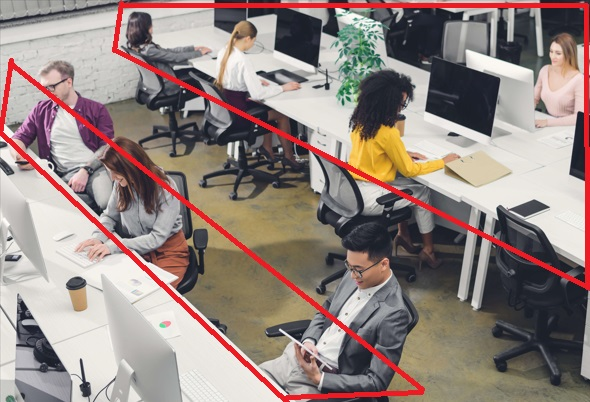
\includegraphics[width=0.5\textwidth]{images/TH2.jpg}
            \caption{Trong trường hợp văn phòng.}
            \label{fig:img_2_VP}
        \end{figure}
        \item Trong sản xuất:\\
        Trong sản xuất, việc các công nhân có làm đúng được vị trí của mình được phân công hay không,...
        \begin{figure}[htbp]
            \centering
            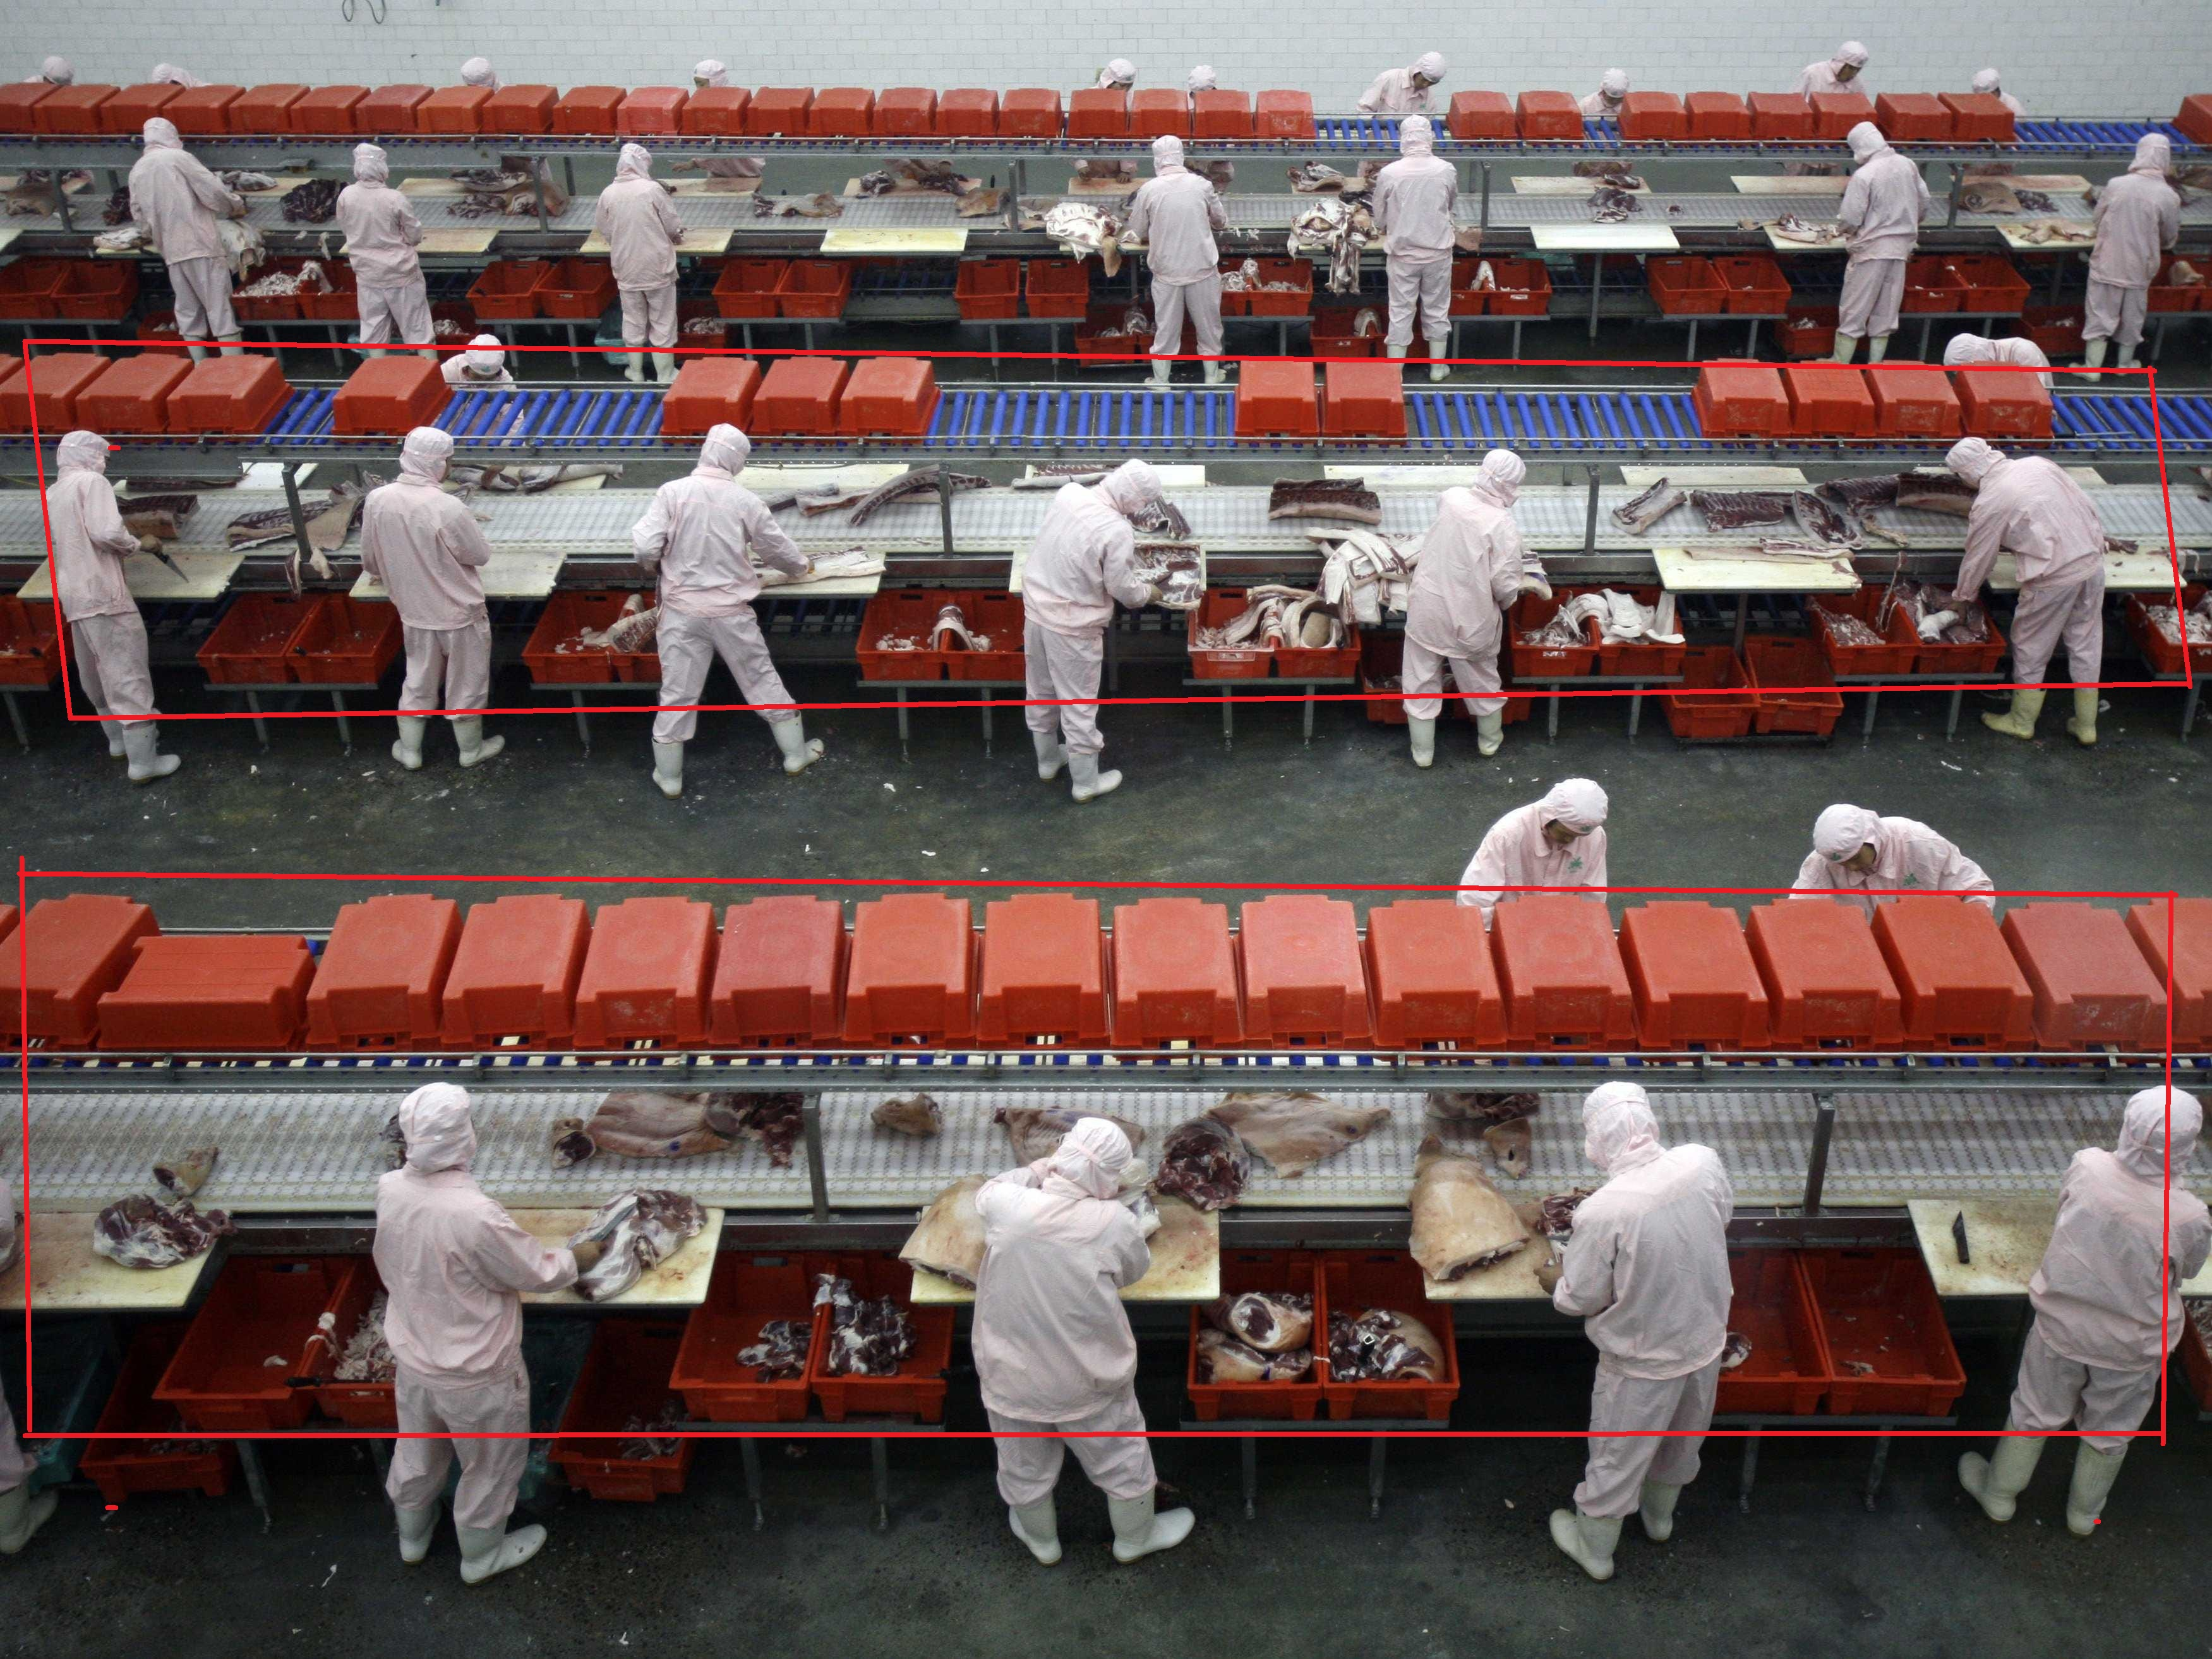
\includegraphics[width=0.5\textwidth]{images/TH3.jpg}
            \caption{Trong trường hợp xí nghiệp.}
            \label{fig:img_3_XN}
        \end{figure}
    \end{itemize}
    

    
    \subsection{Ưu điểm, hạn chế của vấn đề phân tích nêu trên}
    \subsection{Tiến độ thực hiện công việc}
    \subsection{Sơ lược các kỹ thuật, công nghệ liên quan đến các nội dung đã trình bày}
\end{flushleft}
\begin{flushleft}
    \fontsize{16}{20}\selectfont
    \section*{CHƯƠNG 3: CƠ SỞ LÝ THUYẾT}
    \addcontentsline{toc}{section}{CHƯƠNG 3: CƠ SỞ LÝ THUYẾT}
    \fontsize{13}{20}\selectfont
    \setcounter{section}{3}
    \setcounter{subsection}{0}
    \subsection{Giới thiệu về YOLO}
    \fontsize{13}{20}\selectfont\paragraph{}
    YOLO (You Only Look Once) là một trong những thuật toán hàng đầu trong việc nhận diện vật thể. Thuật toán này nổi bật nhờ vào khả năng thực hiện nhận diện rất nhanh chóng và hiệu quả, ngay cả trên những tập dữ liệu lớn và phức tạp. Ý tưởng chính của YOLO là biến bài toán nhận diện vật thể thành một bài toán hồi quy duy nhất, thay vì tiếp cận từng bước như các phương pháp truyền thống.\\
    \begin{figure}[h]
        \centering
        \includegraphics[width=0.5\textwidth]{images/logoYOLO.jpg}
        \caption{Logo YOLOv5}
        \label{fig:logo_YOLO}
    \end{figure}
    \textbf{Nguyên Lý Hoạt Động của YOLO:}\\
    \begin{itemize}
            \item Phân Chia Ảnh: \\Ảnh đầu vào được chia thành một lưới SxS
            \item Dự Đoán Bounding Boxes và Xác Suất:\\Mỗi ô trong lưới dự đoán số lượng các bounding boxes (khung chứa) và xác suất để mỗi khung chứa một vật thể.
            \item Kết Hợp Bounding Boxes: \\Các bounding boxes có xác suất cao sẽ được kết hợp và lọc để đưa ra dự đoán cuối cùng.
    \end{itemize}
    Các phiên bản khác nhau của YOLO (như YOLOv1, YOLOv2, YOLOv3, YOLOv4) đã mang đến nhiều cải tiến về mặt kiến trúc và hiệu năng, nhưng tất cả đều dựa trên nguyên lý cơ bản này.\\
    \textbf{YOLOv5}\\
    YOLOv5 là phiên bản mới của dòng thuật toán YOLO và được phát triển bởi công ty Ultralytics. YOLOv5 kế thừa các ưu điểm của các phiên bản trước và đưa ra nhiều cải tiến quan trọng, cả về mặt tốc độ lẫn độ chính xác.\\
    \textbf{YOLOv5}\\
    \fontsize{13}{20}\selectfont\subsubsection{Các Đặc Điểm Nổi Bật của YOLOv5:}
    \begin{itemize}
        \item Kiến Trúc Nhẹ và Hiệu Quả: YOLOv5 được thiết kế nhẹ nhàng và hiệu quả, cho phép triển khai dễ dàng trên các thiết bị có phần cứng hạn chế.
        \item Cải Tiến về Huấn Luyện: YOLOv5 sử dụng các kỹ thuật mới như Mosaic Augmentation, auto-learning bounding box anchors, và tích hợp sẵn các chiến lược training tốt nhất như cosine learning rate annealing.
        \item Tối Ưu Hóa Hiệu Năng: YOLOv5 có các phiên bản nhỏ gọn (YOLOv5s), trung bình (YOLOv5m), lớn (YOLOv5l), và rất lớn (YOLOv5x) để phù hợp với nhiều loại ứng dụng khác nhau.
        \item Khả Năng Chuyển Giao (Transfer Learning): YOLOv5 hỗ trợ tốt cho việc fine-tuning mô hình trên các tập dữ liệu riêng biệt, giúp dễ dàng tùy chỉnh cho các bài toán cụ thể.
    \end{itemize}
    \fontsize{13}{20}\selectfont\subsubsection{Quá Trình Hoạt Động của YOLOv5}
    \begin{itemize}
        \item Tiền Xử Lý: Ảnh đầu vào được điều chỉnh kích thước và áp dụng các kỹ thuật tăng cường dữ liệu (data augmentation).
        \item Trích Xuất Đặc Trưng: Sử dụng một backbone CNN (như CSPDarknet) để trích xuất các đặc trưng từ ảnh.
        \item Đầu Ra của Mạng: Mạng chia ảnh thành các lưới và dự đoán bounding boxes cùng với xác suất cho từng lưới.
        \item Hậu Xử Lý: Sử dụng các kỹ thuật như Non-Maximum Suppression (NMS) để lọc và kết hợp các bounding boxes, đưa ra dự đoán cuối cùng.
    \end{itemize}
    \fontsize{13}{20}\selectfont\subsubsection{Cải tiến và hiệu năng}
    \begin{itemize}
        \item Tốc Độ và Độ Chính Xác: YOLOv5 vượt trội ở khả năng xử lý ảnh thời gian thực với độ chính xác cao.
        \item Thân Thiện với Người Dùng: Được triển khai bằng PyTorch, YOLOv5 dễ dàng tùy chỉnh và tích hợp vào các hệ thống khác.
        \item Khả Năng Mở Rộng: YOLOv5 có thể mở rộng và tinh chỉnh cho nhiều loại ứng dụng từ giám sát an ninh đến phân tích y tế.
    \end{itemize}
    \subsubsection{Ứng Dụng của YOLOv5}
    \begin{itemize}
        \item Giám Sát An Ninh: Nhận diện các hành vi bất thường hoặc phát hiện kẻ xâm nhập.
        \item Y Tế: Phân tích hình ảnh y tế để phát hiện bệnh tật.
        \item Giao Thông: Phân tích lưu lượng giao thông, nhận diện phương tiện.
        \item Thương Mại Điện Tử: Tự động gán nhãn sản phẩm và quản lý kho hàng.
    \end{itemize}
    YOLOv5 không chỉ tiếp tục di sản của dòng YOLO mà còn mở rộng khả năng của nó, đem lại những tiến bộ vượt bậc trong lĩnh vực nhận diện vật thể. Với sự phát triển liên tục, YOLOv5 hứa hẹn sẽ tiếp tục là công cụ mạnh mẽ và hữu ích cho các ứng dụng trong tương lai.
    \subsection{Giới thiệu về OpenCV}
    OpenCV (Open Source Computer Vision Library) là một thư viện mã nguồn mở mạnh mẽ, được thiết kế để cung cấp các công cụ và giải thuật cho xử lý ảnh và thị giác máy tính. Được phát triển bởi Intel vào năm 1999, OpenCV nhanh chóng trở thành một trong những thư viện phổ biến nhất trong lĩnh vực xử lý ảnh và thị giác máy tính, nhờ tính linh hoạt, hiệu suất cao và khả năng hỗ trợ đa nền tảng.\\
    \begin{figure}[h]
        \centering
        
\includegraphics[width=0.5\textwidth]{images/logoOpenCV.png}
        \caption{Logo OpenCV}
        \label{fig:logo_cv2}
    \end{figure}
    \subsubsection{Các Đặc Điểm Nổi Bật của OpenCV}
    \begin{itemize}
        \item Đa Nền Tảng: Hỗ trợ Windows, Linux, macOS, Android và iOS.
        \item Hỗ Trợ Ngôn Ngữ Đa Dạng: Python, C++, Java và nhiều ngôn ngữ lập trình khác.
        \item Thư Viện Đa Dạng: Cung cấp hơn 2500 thuật toán và hàm xử lý ảnh, bao gồm nhận diện khuôn mặt, phát hiện chuyển động, phân đoạn ảnh, và nhiều hơn nữa.
        \item Hiệu Suất Cao: Được tối ưu hóa cao để sử dụng các phần cứng như CPU và GPU.
    \end{itemize}
    \subsubsection{Vẽ với OpenCV}
    OpenCV cung cấp nhiều hàm vẽ cơ bản để tạo và xử lý các hình ảnh. Các hàm vẽ này bao gồm vẽ đường thẳng, hình chữ nhật, hình tròn, đa giác và thêm văn bản lên ảnh.\\
    \begin{itemize}
        \item cv2.line(): Vẽ đường thẳng.
        \item cv2.rectangle(): Vẽ hình chữ nhật.
        \item cv2.circle(): Vẽ hình tròn.
        \item cv2.ellipse(): Vẽ hình ellipse.
        \item cv2.polylines(): Vẽ đa giác.
        \item cv2.putText(): Thêm văn bản lên ảnh.
    \end{itemize}
    \subsubsection{Các Bước Thao Tác với Camera}
    \begin{itemize}
        \item Mở Camera: Sử dụng cv2.VideoCapture() để mở camera.
        \item Đọc Khung Hình: Sử dụng cap.read() để đọc từng khung hình từ camera.
        \item Thị Khung Hình: Sử dụng cv2.imshow() để hiển thị khung hình.
        \item Lý Khung Hình: Áp dụng các thuật toán xử lý ảnh lên từng khung hình.
        \item Video: Sử dụng cv2.VideoWriter() để lưu lại video nếu cần.
    \end{itemize}
    \subsubsection{Ứng Dụng của OpenCV}
    OpenCV được sử dụng rộng rãi trong nhiều lĩnh vực khác nhau: \\
    Giám Sát An Ninh: Phát hiện chuyển động, nhận diện khuôn mặt.
    Y Tế: Phân tích hình ảnh y tế, nhận diện bệnh lý.
    Giao Thông: Phân tích lưu lượng giao thông, nhận diện biển số xe.
    Thương Mại Điện Tử: Quản lý kho hàng, phân loại sản phẩm.


\end{flushleft}

\begin{flushleft}
    \fontsize{16}{20}\selectfont
    \section*{KẾT LUẬN}
    \addcontentsline{toc}{section}{KẾT LUẬN}
    \setcounter{section}{5}
    \setcounter{subsection}{0}
\end{flushleft}
\begin{flushleft}
    \fontsize{16}{20}\selectfont
    \section*{TÀI LIỆU THAM KHẢO}
    \addcontentsline{toc}{section}{TÀI LIỆU THAM KHẢO}
    \setcounter{section}{6}
    \setcounter{subsection}{0}
    \printbibliography
\end{flushleft}
\end{document}
